\documentclass[aspectratio=169]{beamer}
\usepackage{amsmath}
\usepackage{amssymb}
\usepackage{tikz}
\usepackage{xcolor}
\usetikzlibrary{shapes,backgrounds,patterns}

\usepackage{pgfplots}
\pgfplotsset{compat=1.18, legend cell align=left}
\usetikzlibrary{arrows.meta,decorations.pathreplacing,calc,positioning}
\usepackage{booktabs}
\usepackage{pifont}
\usepgfplotslibrary{fillbetween}

% royalblue isn't a base xcolor name, so define it first (this is the default accent)
\definecolor{royalblue}{RGB}{65,105,225}

% ============================================================
%  ACCENT COLOR: change ONE line below to switch the theme
%  Choose one of: royalblue , red , black
% ============================================================
\colorlet{accent}{royalblue}
% \colorlet{accent}{red}
% \colorlet{accent}{black}
% ============================================================

% colorblind-safe, high-contrast second color (Okabe-Ito vermillion)
\definecolor{hl}{RGB}{213,94,0}

\usetheme{default}
\setbeamercolor{background canvas}{bg=white}
\setbeamercolor{normal text}{fg=black}
\setbeamercolor{structure}{fg=accent}
\setbeamercolor{frametitle}{fg=accent,bg=white}
\setbeamercolor{title}{fg=accent}
\setbeamercolor{section in toc}{fg=black}
\setbeamercolor{block title}{fg=black,bg=gray!10}
\setbeamercolor{block body}{fg=black,bg=gray!5}
\setbeamercolor{block title example}{fg=black,bg=green!10}
\setbeamercolor{block body example}{fg=black,bg=green!5}
\setbeamercolor{block title alerted}{fg=black,bg=red!10}
\setbeamercolor{block body alerted}{fg=black,bg=red!5}

\setbeamertemplate{navigation symbols}{}
\setbeamertemplate{footline}{
    \hfill\makebox[5pt]{%
        \scriptsize\insertframenumber}
    \hspace*{2em}
    \vspace{0.5cm}
}

\newcommand{\cbox}[2]{\colorbox{#1}{\ensuremath{\displaystyle #2}}}

\pgfplotsset{
  miniplot/.style={
    width=4.0cm, height=3.0cm,
    axis lines=middle, xtick=\empty, ytick=\empty,
    samples=120, thick, clip=true
  }
}

\definecolor{gr}{RGB}{0,158,115}

\title{Finite Differences: Summary}
\subtitle{Derivatives from function values}
\author{Sharareh Sayyad}
\institute{Washington State University}
\date{\today}

\pgfmathdeclarefunction{g}{1}{\pgfmathparse{0.25*#1^2+0.3*sin(deg(2*#1))+0.6}}
\pgfmathdeclarefunction{gp}{1}{\pgfmathparse{0.5*#1+0.6*cos(deg(2*#1))}}

\begin{document}
\frame{\titlepage}

% ------------------------------------------------------------
\begin{frame}{The task}
\begin{columns}[T]
\begin{column}{0.46\textwidth}
\small
\begin{block}{Given only values of $f$}
Approximate the slope at $x$:
\[
\cbox{gray!15}{f'(x) = \lim_{h\to 0}\frac{f(x+h)-f(x)}{h}}
\]
\end{block}
\begin{itemize}
\item Take a \textbf{small step} $h$: a \textbf{secant} instead of the tangent.
\item No formula for $f'$ needed: only \textbf{evaluations} of $f$.
\end{itemize}
\footnotesize
All formulas come from Taylor's theorem:
\[ f(x\pm h) = f \pm h f' + \tfrac{h^2}{2} f'' \pm \tfrac{h^3}{6} f''' + \dots \]
\end{column}
\begin{column}{0.52\textwidth}
\centering
\begin{tikzpicture}
\begin{axis}[width=7.5cm,height=5.4cm,axis lines=left,xmin=0.2,xmax=3.0,ymin=0.6,ymax=3.0,
  xtick={0.9,1.6,2.3},xticklabels={$x-h$,$x$,$x+h$},ytick=\empty,thick,
  legend style={font=\scriptsize,at={(0.02,0.98)},anchor=north west}]
\addplot[black,domain=0.3:2.9,samples=80,forget plot] {g(x)};
\addplot[black!60,domain=0.5:2.9,samples=2] {g(1.6)+gp(1.6)*(x-1.6)};
\addplot[accent,domain=0.9:2.9,samples=2] {g(1.6)+(g(2.3)-g(1.6))/0.7*(x-1.6)};
\addplot[hl,dashed,domain=0.5:2.3,samples=2] {g(1.6)+(g(1.6)-g(0.9))/0.7*(x-1.6)};
\addplot[gr,densely dotted,very thick,domain=0.5:2.9,samples=2] {g(0.9)+(g(2.3)-g(0.9))/1.4*(x-0.9)};
\addplot[only marks,mark=*,black,mark size=1.8pt] coordinates {(0.9,{g(0.9)}) (1.6,{g(1.6)}) (2.3,{g(2.3)})};
\legend{tangent (exact), forward, backward, central}
\end{axis}
\end{tikzpicture}

\footnotesize The central secant is almost \textbf{parallel} to the tangent.
\end{column}
\end{columns}
\end{frame}

% ------------------------------------------------------------
\begin{frame}{Four formulas}
\centering
\small
\setlength{\tabcolsep}{10pt}\renewcommand{\arraystretch}{1.3}
\begin{tabular}{@{}lll@{}}
\toprule
name & formula & error \\ \midrule\addlinespace[4pt]
\textcolor{accent}{\textbf{forward}} & $\dfrac{f(x+h)-f(x)}{h}$ & $O(h)$ \\[7pt]
\textcolor{hl}{\textbf{backward}} & $\dfrac{f(x)-f(x-h)}{h}$ & $O(h)$ \\[7pt]
\textcolor{gr}{\textbf{central}} & $\dfrac{f(x+h)-f(x-h)}{2h}$ & $O(h^2)$ \\[7pt]
\textbf{5-point} & $\dfrac{-f(x+2h)+8f(x+h)-8f(x-h)+f(x-2h)}{12h}$ & $O(h^4)$ \\
\bottomrule
\end{tabular}

\vspace{0.3em}
\footnotesize
\begin{minipage}{0.80\textwidth}
\begin{itemize}
\item forward / backward: error $\approx \pm\frac{h}{2}f''$, \textbf{opposite signs}
\item central = their average $\Rightarrow$ the $f''$ terms \textbf{cancel}, error $\approx \frac{h^2}{6}f'''$
\item 5-point: combine steps $h$ and $2h$ $\Rightarrow$ the $h^2$ terms cancel too
\end{itemize}
\end{minipage}

\vspace{0.3em}
\cbox{accent!12}{\text{Order } O(h^p)\text{: halve } h \;\Rightarrow\; \text{error} \div 2^p}
\end{frame}

% ------------------------------------------------------------
\begin{frame}{Choosing $h$: two errors pull in opposite directions}
\begin{columns}[T]
\begin{column}{0.54\textwidth}
\centering
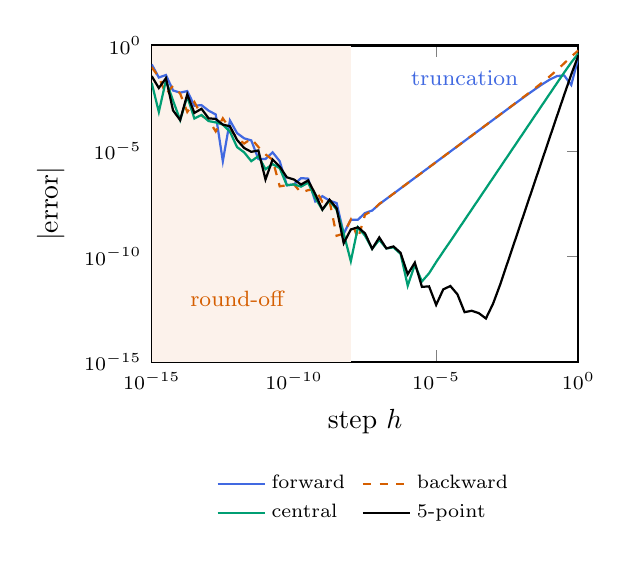
\begin{tikzpicture}
\begin{axis}[width=7.0cm,height=5.6cm,xmode=log,ymode=log,xmin=1e-15,xmax=1,ymin=1e-15,ymax=1,
  xlabel={step $h$},ylabel={$|$error$|$},thick,tick label style={font=\scriptsize},
  xtick={1e-15,1e-10,1e-5,1},ytick={1e-15,1e-10,1e-5,1},
  legend style={font=\scriptsize,at={(0.5,-0.32)},anchor=north,legend columns=2,draw=none,/tikz/every even column/.append style={column sep=4pt}}]
\fill[hl!8] (axis cs:1e-15,1e-15) rectangle (axis cs:1e-8,1);
\addplot[accent] coordinates {(1.000e-15,1.280e-01) (1.778e-15,3.051e-02) (3.162e-15,4.003e-02) (5.623e-15,7.419e-03) (1.000e-14,5.844e-03) (1.778e-14,6.953e-03) (3.162e-14,1.408e-03) (5.623e-14,1.496e-03) (1.000e-13,8.174e-04) (1.778e-13,5.393e-04) (3.162e-13,3.299e-06) (5.623e-13,2.806e-04) (1.000e-12,7.079e-05) (1.778e-12,3.985e-05) (3.162e-12,3.181e-05) (5.623e-12,4.187e-06) (1.000e-11,4.180e-06) (1.778e-11,8.634e-06) (3.162e-11,3.299e-06) (5.623e-11,2.381e-07) (1.000e-10,2.610e-07) (1.778e-10,5.175e-07) (3.162e-10,4.906e-07) (5.623e-10,4.070e-08) (1.000e-09,7.210e-08) (1.778e-09,4.440e-08) (3.162e-09,3.415e-08) (5.623e-09,1.218e-09) (1.000e-08,5.491e-09) (1.778e-08,5.547e-09) (3.162e-08,1.149e-08) (5.623e-08,1.504e-08) (1.000e-07,2.992e-08) (1.778e-07,5.362e-08) (3.162e-07,9.470e-08) (5.623e-07,1.690e-07) (1.000e-06,3.001e-07) (1.778e-06,5.337e-07) (3.162e-06,9.492e-07) (5.623e-06,1.688e-06) (1.000e-05,3.002e-06) (1.778e-05,5.338e-06) (3.162e-05,9.492e-06) (5.623e-05,1.688e-05) (1.000e-04,3.001e-05) (1.778e-04,5.336e-05) (3.162e-04,9.487e-05) (5.623e-04,1.686e-04) (1.000e-03,2.996e-04) (1.778e-03,5.321e-04) (3.162e-03,9.439e-04) (5.623e-03,1.671e-03) (1.000e-02,2.948e-03) (1.778e-02,5.168e-03) (3.162e-02,8.953e-03) (5.623e-02,1.517e-02) (1.000e-01,2.454e-02) (1.778e-01,3.581e-02) (3.162e-01,3.826e-02) (5.623e-01,1.350e-02) (1.000e+00,2.656e-01)};
\addplot[hl,dashed] coordinates {(1.000e-15,9.408e-02) (1.778e-15,3.193e-02) (3.162e-15,4.918e-03) (5.623e-15,1.232e-02) (1.000e-14,5.258e-03) (1.778e-14,7.093e-04) (3.162e-14,2.103e-03) (5.623e-14,4.780e-04) (1.000e-13,2.928e-04) (1.778e-13,8.501e-05) (3.162e-13,3.544e-04) (5.623e-13,1.143e-04) (1.000e-12,4.023e-05) (1.778e-12,2.258e-05) (3.162e-12,3.841e-05) (5.623e-12,1.556e-05) (1.000e-11,6.922e-06) (1.778e-11,3.853e-06) (3.162e-11,2.116e-07) (5.623e-11,2.381e-07) (1.000e-10,2.610e-07) (1.778e-10,1.068e-07) (3.162e-10,1.395e-07) (5.623e-10,1.567e-07) (1.000e-09,3.892e-08) (1.778e-09,4.440e-08) (3.162e-09,9.589e-10) (5.623e-09,1.218e-09) (1.000e-08,5.611e-09) (1.778e-08,6.963e-10) (3.162e-08,9.574e-09) (5.623e-08,1.458e-08) (1.000e-07,3.115e-08) (1.778e-07,5.314e-08) (3.162e-07,9.524e-08) (5.623e-07,1.688e-07) (1.000e-06,3.002e-07) (1.778e-06,5.338e-07) (3.162e-06,9.492e-07) (5.623e-06,1.688e-06) (1.000e-05,3.002e-06) (1.778e-05,5.338e-06) (3.162e-05,9.493e-06) (5.623e-05,1.688e-05) (1.000e-04,3.002e-05) (1.778e-04,5.340e-05) (3.162e-04,9.498e-05) (5.623e-04,1.690e-04) (1.000e-03,3.007e-04) (1.778e-03,5.355e-04) (3.162e-03,9.546e-04) (5.623e-03,1.705e-03) (1.000e-02,3.055e-03) (1.778e-02,5.506e-03) (3.162e-02,1.002e-02) (5.623e-02,1.855e-02) (1.000e-01,3.521e-02) (1.778e-01,6.940e-02) (3.162e-01,1.429e-01) (5.623e-01,3.017e-01) (1.000e+00,5.829e-01)};
\addplot[gr] coordinates {(1.000e-15,1.695e-02) (1.778e-15,7.093e-04) (3.162e-15,2.247e-02) (5.623e-15,2.452e-03) (1.000e-14,2.928e-04) (1.778e-14,3.831e-03) (3.162e-14,3.478e-04) (5.623e-14,5.091e-04) (1.000e-13,2.623e-04) (1.778e-13,2.271e-04) (3.162e-13,1.788e-04) (5.623e-13,8.316e-05) (1.000e-12,1.528e-05) (1.778e-12,8.634e-06) (3.162e-12,3.299e-06) (5.623e-12,5.685e-06) (1.000e-11,1.371e-06) (1.778e-11,2.390e-06) (3.162e-11,1.544e-06) (5.623e-11,2.381e-07) (1.000e-10,2.610e-07) (1.778e-10,2.053e-07) (3.162e-10,3.150e-07) (5.623e-10,5.801e-08) (1.000e-09,1.659e-08) (1.778e-09,4.440e-08) (3.162e-09,1.660e-08) (5.623e-09,1.218e-09) (1.000e-08,5.963e-11) (1.778e-08,2.425e-09) (3.162e-08,9.589e-10) (5.623e-08,2.309e-10) (1.000e-07,6.147e-10) (1.778e-07,2.402e-10) (3.162e-07,2.699e-10) (5.623e-07,1.322e-10) (1.000e-06,4.119e-12) (1.778e-06,4.074e-11) (3.162e-06,6.553e-12) (5.623e-06,1.591e-11) (1.000e-05,5.408e-11) (1.778e-05,1.719e-10) (3.162e-05,5.314e-10) (5.623e-05,1.692e-09) (1.000e-04,5.347e-09) (1.778e-04,1.691e-08) (3.162e-04,5.347e-08) (5.623e-04,1.691e-07) (1.000e-03,5.347e-07) (1.778e-03,1.691e-06) (3.162e-03,5.347e-06) (5.623e-03,1.691e-05) (1.000e-02,5.347e-05) (1.778e-02,1.691e-04) (3.162e-02,5.345e-04) (5.623e-02,1.690e-03) (1.000e-01,5.335e-03) (1.778e-01,1.679e-02) (3.162e-01,5.230e-02) (5.623e-01,1.576e-01) (1.000e+00,4.243e-01)};
\addplot[black] coordinates {(1.000e-15,3.545e-02) (1.778e-15,9.696e-03) (3.162e-15,2.832e-02) (5.623e-15,8.382e-04) (1.000e-14,2.928e-04) (1.778e-14,4.872e-03) (3.162e-14,6.404e-04) (5.623e-14,1.003e-03) (1.000e-13,3.548e-04) (1.778e-13,3.312e-04) (3.162e-13,1.788e-04) (5.623e-13,1.490e-04) (1.000e-12,3.379e-05) (1.778e-12,1.384e-05) (3.162e-12,9.151e-06) (5.623e-12,1.062e-05) (1.000e-11,4.460e-07) (1.778e-11,3.951e-06) (3.162e-11,1.836e-06) (5.623e-11,5.672e-07) (1.000e-10,4.460e-07) (1.778e-10,2.574e-07) (3.162e-10,4.028e-07) (5.623e-10,9.092e-08) (1.000e-09,1.659e-08) (1.778e-09,4.960e-08) (3.162e-09,1.952e-08) (5.623e-09,4.272e-10) (1.000e-08,1.910e-09) (1.778e-08,2.425e-09) (3.162e-08,1.251e-09) (5.623e-08,2.309e-10) (1.000e-07,7.998e-10) (1.778e-07,2.402e-10) (3.162e-07,2.991e-10) (5.623e-07,1.486e-10) (1.000e-06,1.438e-11) (1.778e-06,5.115e-11) (3.162e-06,3.627e-12) (5.623e-06,3.833e-12) (1.000e-05,5.071e-13) (1.778e-05,2.764e-12) (3.162e-05,3.979e-12) (5.623e-05,1.596e-12) (1.000e-04,2.294e-13) (1.778e-04,2.671e-13) (3.162e-04,2.052e-13) (5.623e-04,1.152e-13) (1.000e-03,5.755e-13) (1.778e-03,4.643e-12) (3.162e-03,4.676e-11) (5.623e-03,4.679e-10) (1.000e-02,4.679e-09) (1.778e-02,4.678e-08) (3.162e-02,4.678e-07) (5.623e-02,4.675e-06) (1.000e-01,4.666e-05) (1.778e-01,4.637e-04) (3.162e-01,4.547e-03) (5.623e-01,4.265e-02) (1.000e+00,3.405e-01)};
\legend{forward, backward, central, 5-point}
\node[font=\footnotesize,hl] at (axis cs:1e-12,1e-12) {round-off};
\node[font=\footnotesize,accent] at (axis cs:1e-4,3e-2) {truncation};
\end{axis}
\end{tikzpicture}
\end{column}
\begin{column}{0.44\textwidth}
\small
\begin{block}{Large $h$: truncation error}
\footnotesize Error $\propto h^p$: falls as $h$ shrinks.
\end{block}
\begin{block}{Small $h$: round-off error}
\footnotesize $f(x+h) \approx f(x)$: the subtraction loses digits. Error $\propto 1/h$: grows as $h$ shrinks.
\end{block}

\vspace{0.3em}
\footnotesize
Each curve is a \textbf{V}: the \textbf{best $h$} is at the bottom.

\vspace{0.4em}
\centering
\begin{tabular}{@{}lll@{}}
\toprule
formula & best $h$ & best error \\ \midrule
forward, backward & $10^{-8}$ & $10^{-8}$ \\
central & $10^{-5}$ & $10^{-11}$ \\
5-point & $10^{-3}$ & $10^{-13}$ \\
\bottomrule
\end{tabular}
\end{column}
\end{columns}
\end{frame}

% ------------------------------------------------------------
\begin{frame}{Take-home}
\begin{columns}[T]
\begin{column}{0.48\textwidth}
\begin{exampleblock}{Finite differences}
\small
\begin{itemize}
\item Need only \textbf{values} of $f$, no formula.
\item Forward, backward: $O(h)$. Central: $O(h^2)$. 5-point: $O(h^4)$.
\item Symmetric formulas cancel error terms: use \textbf{central} or \textbf{5-point}.
\end{itemize}
\end{exampleblock}
\end{column}
\begin{column}{0.48\textwidth}
\begin{alertblock}{Choosing $h$}
\small
\begin{itemize}
\item Too large: \textbf{truncation} error.
\item Too small: \textbf{round-off} error.
\item Best $h$ is in between; never exact.
\item Check against an exact derivative (SymPy) when you can.
\end{itemize}
\end{alertblock}
\end{column}
\end{columns}
\vspace{0.8em}
\centering
\cbox{accent!12}{\text{A derivative from values: pick the formula, then pick } h \text{ with care.}}
\end{frame}

\end{document}
